\documentclass{VUMIFPSkursinis}
\usepackage{algorithmicx}
\usepackage{algorithm}
\usepackage{algpseudocode}
\usepackage{amsfonts}
\usepackage{amsmath}
\usepackage{bm}
\usepackage{caption}
\usepackage{color}
\usepackage{float}
\usepackage{graphicx}
\usepackage{listings}
\usepackage{subfig}
\usepackage{wrapfig}
\usepackage{multirow}
\usepackage{longtable}
\usepackage{array,makecell}

% Titulinio aprašas
\university{Vilniaus universitetas}
\faculty{Matematikos ir informatikos fakultetas}
\department{Programų sistemų katedra}
\papertype{Programų sistemų inžinerija: 3 laboratorinis darbas}
\title{Stalo žaidimų programėlė}
\titleineng{Board Games Application}
\status{2 kurso 5 grupės studentai}
\author{Elena Reivytytė}
\secondauthor{Matas Šilinskas}
\thirdauthor{Kasparas Taminskas}
\fourthauthor{Aidas Vaikšnoras}
\fifthauthor{Tadas Žaliauskas}
\supervisor{dr. Vytautas Valaitis}
\date{Vilnius – \the\year}

% Nustatymai
% \setmainfont{Palemonas}   % Pakeisti teksto šriftą į Palemonas (turi būti įdiegtas sistemoje)
\bibliography{bibliografija}

\begin{document}
\maketitle

\sectionnonum{Anotacija}
Šis darbas yra skirtas aprašyti stalo žaidimų mobiliosios programėlės vidinei ir išorinei analizei. 
Programėlės tikslas yra suvienyti žmones, esančius artimoje aplinkoje ir mėgstančius žaisti stalo žaidimus. 
Mobiliosios programėles tikslinė auditorija yra žmonės, mėgstantys stalo žaidimus, esantys tam 
tikrose uždarose grupėse (pvz. butų, bendrabučių gyventojai ar festivalių dalyviai) ieškantys žaidėjų stalo žaidimams. 

\tableofcontents

\section{Įvadas}
\textbf{Darbo tikslas}\\
Išanalizuoti esamą stalo žaidimų organizavimo rinką ir pasitelkus analizę sukurti naują projektą, 
gebantį sujungti žmones bendram laisvalaikio praleidimui žaidžiant stalo žaidimus, pasitelkiant 
inovatyvias idėjas ir pateikti sprendimą, pagelbėsiantį trūkstamų žaidimo draugų paieškoje.

\textbf{Temos aktualumas}\\
Stalo žaidimai, kaip alternatyva kompiuteriniams žaidimams, išlaiko gausų gerbėjų ratą - tai 
yra žmones, kurie vertina gyvą bendravimą. Be to ši žaidėjų auditorija yra itin tikslinė ir 
lojali. Bendrabučiuose ir festivaliuose žmonės dažnai buriasi į grupeles smagiai praleisti 
laisvalaikį prie žaidimų lentos. Iki šiol stalo žaidimų organizavimu vertėsi tik specializuotos 
kavinės, tačiau tokių kavinių mastas yra mažas, o žaidimai vykdavo gana retai, organizatorių 
nustatytoje vietoje, tad reikėdavo papildomai keliauti iš namų. Tačiau iškyla problema, kaip, 
žaidimui pritrūkus žmonių, visiškai nepažįstami žmonės irgi galėtų būti įtraukti į tokį laisvalaikio 
praleidimo būdą. Į pagalbą ateitų mūsų programėlė, kuri leistų atrasti planuojamus žaisti stalo 
žaidimus aplink ir prie jų prisijungti pateikus prašymą.

\textbf{Siekiami rezultatai}\\
Mes siekiame padidinti žmonių susidomėjimą stalo žaidimais, skatiname juos rinktis tokią veiklą 
ir sukurti stalo žaidimus apjungiančią sistemą. Tikimasi, kad mėgėjai aktyviai kurs ir kvies 
kitus prisijungti prie stalo žaidimų, o nerandantys su kuo žaisti, atras sau žaidimo draugų. 
Siekiame, kad programėlė pritrauktų ir žaidimų platintojus plačiai reklamuotis programėlėje, 
kurie siūlytų išbandyti naujus, didelio susidomėjimo sulaukusius žaidimus už teikiamą paramą mums.

\section{Verslo proceso aprašymas}
Nagrinėjama verslas - stalo žaidimai. Jie dažniausiai žaidžiami ant žaidimo 
lentos ar kitaip pažymėto žaidimo ploto su specialiais žaidimo komponentais 
(kauliukai, figūrėlės, kortelės).

\textbf{Nagrinėjamos srities apibrėžimas:}\\
Stalo žaidimai, įdomus ir linksmas laisvalaikio praleidimo būdas, aktyvus 
laisvalaikis, pramogos

\textbf{Dalykinė sritis:}\\
Stalo žaidimai ir pagalba juos organizuojant

\textbf{Probleminė sritis:}\\
Plataus spektro stalo žaidimų organizavimas, yra žaidėjų, kurie organizuoja 
žaidimą, tačiau jiems trūksta žaidėjų, kad žaidimas įvyktų, taip pat yra žmonių, 
kurie nori žaisti konkretų žaidimą, bet neturi draugų, norinčių žaisti tą žaidimą.

Daugeliui, išgirdus žodį „stalo žaidimai“, galvoje sukuriama asociacija 
su vaikais ar paaugliais. Tačiau stalo žaidimų yra labai daug ir įvairių, 
sukurtų skirtingoms amžiaus grupėms, reikalaujančių skirtingų žaidėjo savybių 
(strateginis mąstymas, diplomatiniai sugebėjimai, rankų miklumas, kūrybiniai 
gebėjimai) ir naudojančių skirtingus žaidimo komponentus. Dauguma net nesusimąsto, 
kad stalo žaidimai turi ir mokomąja vertę. Tarp gausybės spalvingų žaidimų galima 
rasti tokių, kurie vysto vaiko raidą, padeda pažinti raides ir mokytis skaityti, 
lavina matematinius, loginius bei kūrybinius įgūdžius. Vis dažniau prie stalo 
žaidimų galima sutikti ir vyresnių, net ir garbaus amžiaus žmonių, susižavėjusių 
šia turininga ir užkrečiančia pramoga, kuri tampa lyg šeimos tradicija susirinkti 
prie bendro stalo. Neretai kalbant apie stalo žaidimus omenyje taip pat turimi ir 
klasikiniai žaidimai (šachmatai, šaškės, domino), kortų žaidimai ar vaidmenų žaidimai.\\
Ilgą laiką beveik išimtinai aukštuomenės pramoga buvę stalo žaidimai, kaip idealus 
šeimos laisvalaikio leidimo būdas, išpopuliarėjo JAV XX amžiaus viduryje. 
Didžiausias pagyvėjimas po vėliau prarastų pozicijų kompiuteriniams ir konsolių 
žaidimams, „gyvų“ žaidimų rinkoje buvo juntamas 9-ajame dešimtmetyje, atsiradus 
kolekcionuojamiems kortų žaidimams ir padidėjus modernių stalo žaidimų populiarumui.\\
Savo mobiliąja programėle stengsimės padidinti stalo žaidimų populiarumą suteikiant 
geresnes sąlygas siekiant surasti trūkstamų žaidėjų skaičių, kitaip tariant 
supaprastinant žaidimo organizavimo procesą, kuris be tokios platformos yra gana 
keblus, nes žaidimui reikia neretai 4-10 žaidėjų, kurie būtų pasiruošė paskirti 
pora valandų žaidimo sesijai.

\section{Išorinė proceso analizė}
	\subsection{Dabartinio verslo sistemos įeiga:}
		\renewcommand{\labelitemi}{$\bullet$}
			\begin{itemize}
				\item Žaidėjo registracijos duomenys. Ši įeiga pasirinkta todėl, 
				kad ji yra būtina šiuolaikiniame versle. Žaidėjai, neįvedę 
				registracijos duomenų - vardo, pavardės, prisijungimo vardo, 
				elektroninio pašto - negali naudotis programėle. Dėl saugumo tikslų 
				taip pat galima pateikti nuotrauką taip parodant, kad naudotojas 
				nebijo atskleisti savo tapatybės kitiems žaidėjams.
				\item Rėmėjai (stalo žaidimų prekyba užsiimantys verslai).
				\item Žaidėjai, kuriantys žaidimų sesijas.
				\item Stalo žaidimų klubai (pvz. RIKIS).
			\end{itemize}
	\subsection{Dabartinio verslo sistemos išeiga:}
		\renewcommand{\labelitemi}{$\bullet$}
			\begin{itemize}
				\item Žaidimo, laukimo laikas ir atstumas iki žaidimo vietos. 
				Šios charakteristikos pasirinktos tam, kad vartotojas galėtų 
				nustatyti, ar verta prisijungti ir dalyvauti žaidime. Vartotojas 
				gali pasirinkti nedalyvauti žaidime, kuris yra toli nuo jo namų 
				arba jo žaidimo/ laukimo iki pradžios laikas yra per didelis.
				\item Sėkmingai įvykę stalo žaidimų susibūrimai.
				\item Prizai, skatinantys dalyvių aktyvumą.
				\item Žaidėjų atsiliepimai, palikti po įvykusio stalo žaidimo.
			\end{itemize}
	\subsection{Dabartinis verslas reguliuojamas šių taisyklių:}
		\renewcommand{\labelitemi}{$\bullet$}
			\begin{itemize}
				\item Viešai atskleisti trečiosioms šalims ar naudoti pateiktus 
				vartotojo duomenis be jo sutikimo yra draudžiama.
				\item Ribotas kapitalo kiekis veiklos pradžioje.
			\end{itemize}
	\subsection{Dabartinis verslo įvaizdžio formavimas:}
		\renewcommand{\labelitemi}{$\bullet$}
			\begin{itemize}
				\item Atsiliepimai internete,
				\item Reklama socialiniuose tinkluose.
				\item Rėmėjų steigiami prizai.
				\item Remėjų rengiami konkursai ir varžybos.
			\end{itemize}
			
	\subsection{Įeigos metrikos}			
		\begin{longtable}{ | m{3.5cm} | m{3.5cm} | m{3.5cm} | >{\centering}m{1.6cm} | >{\centering}m{1.6cm} | }
		\caption{Įeigos metrikos}
		\label{variability_impl_mech}
		%\endfirsthead
		\endhead
		 \hline			

		\centering{\textbf{Metrika}} & \centering{\textbf{Matavimo vienetas}} & \textbf{Kaip matuoti} & \textbf{Dabartinė reikšmė} & \textbf{Kritinė reikšmė} \tabularnewline \hline
		Žaidėjo registracijos duomenys. & Procentas žaidėjų, kurie pateikė vardą. & Suskaičiuoti dalį žaidėjų, kurie pateikė vardą. & 100\% & 100\% \tabularnewline \hline
		Žaidėjo registracijos duomenys. & Procentas žaidėjų, kurie pateikė pavardę. & Suskaičiuoti dalį žaidėjų, kurie pateikė pavardę. & 100\% & 100\% \tabularnewline \hline
		Žaidėjo registracijos duomenys. & Procentas žaidėjų, kurie pateikė prisijungimo vardą. & Suskaičiuoti dalį žaidėjų, kurie pateikė prisijungimo vardą. & 100\% & 100\% \tabularnewline \hline
		Žaidėjo registracijos duomenys. & Procentas žaidėjų, kurie pateikė elektroninį paštą. & Suskaičiuoti dalį žaidėjų, kurie pateikė elektroninį paštą. & 100\% & 100\% \tabularnewline \hline
		Žaidėjo registracijos duomenys. & Procentas žaidėjų, kurie pateikė nuotrauką. & Suskaičiuoti dalį žaidėjų, kurie pateikė nuotrauką. & 50\% & 50\% \tabularnewline \hline
		Atstumas nuo žaidėjo iki žaidimo vietos. & Vidutinis nukeliaujamas atstumas nuo žaidėjo iki žaidimo vietos. & Suskaičiuoti visų žaidėjų, išskyrus žaidimo kūrėjų, kiekvieno žaidimo nuvyktą atstumą ir išvesti vidurkį. & 0.8 km & 1.0 km \tabularnewline \hline
		Žaidimo trukmė. & Vidutinė žaidimo trukmė valandomis. & Suskaičiuoti vykusių žaidimų trukmes ir išvesti vidurkį. & 3.5 h & 4.0 h \tabularnewline \hline
		Laukimo trukmė. & Vidutinė laukimo iki žaidimo pradžios trukmė valandomis. & Suskaičiuoti laukimo iki žaidimų pradžių trukmes ir išvesti vidurkį. & 1.5 h & 1.0 h \tabularnewline \hline
		Vartotojo pateikiamas mokestis už žaidimo iškėlimą. & Procentas vartotojų, kurie pirko paslaugą. & Suskaičiuoti, dalį vartotojų, kurie naudojosi mokama paslauga iškelti žaidimą visų sąraše, o kiek nemokama. & Mokama: 1\% Nemokama: 99\% & Mokama: 5 \% Nemokama: 95 \% \tabularnewline \hline
		Žaidimų duomenys. & Visų įvykusių žaidimų skaičius. & Suskaičiuoti visų įvykusių žaidimų skaičių. & 60\% & 80\% \tabularnewline \hline
		Žaidimų duomenys. & Visų neįvykusių žaidimų skaičius. & Suskaičiuoti visų neįvykusių žaidimų skaičių. & 40\% & 20\% \tabularnewline \hline
		Žaidimų duomenys. & Vidutinis žmonių kiekis žaidime. & Suskaičiuoti visų įvykusių žaidimų žaidėjų skaičių ir išvesti vidurkį. & 6 & 6 \tabularnewline \hline
		Žaidimų duomenys. & Aktyvių programėlės naudotojų, dalyvaujančių žaidimuose, skaičius. & Suskaičiuoti žaidėjus, kurie per savaitę sužaidžia bent vieną žaidimą. & 0 & 1000 \tabularnewline \hline
		Žaidimų duomenys. & Vidutinis asmeninių išsiųstų žinučių kiekis per mėnesį. & Suskaičiuoti visų asmeninių išsiųstų žaidėjų žinutes ir išvesti vidurkį. & 75 & 100 \tabularnewline \hline
		Žaidimų duomenys. & Vidutinis išsiųstų žinučių kiekis žaidimo kūrimo lange per mėnesį. & Suskaičiuoti visų išsiųstų žaidėjų žinutes žaidimo kūrimo lange ir išvesti vidurkį. & 325 & 500 \tabularnewline \hline
		Rėmėjų duomenys. & Rėmėjų, užsiimančių žaidimų prekyba ir norinčių remti programėlę mainais už reklamą, skaičius. & Suskaičiuoti visus rėmėjus, užsiimančius žaidimų prekyba ir norinčius remti programėlę mainais už reklamą. & 0 & 7 \tabularnewline \hline
		Rėmėjų duomenys. & Remėjų, užsiregistravusių programėlėje ir reklamuojančių savo prekes, sukurtų prekės pristatymo renginių vidurkis. & Suskaičiuoti, kiek renginių kiekviena kompanija inicijuoja ir išvesti vidurkį. & 0 & <5 \tabularnewline \hline
		Rėmėjų duomenys. & Vidutinis skaičius žaidėjų, sekančių užsiregistravusį remėją. & Suskaičiuoti, kiek žaidėjų seka kiekvieną užsiregistravusį remėją ir išvesti vidurkį. & 0 & <5 \tabularnewline \hline
	    \end{longtable}
		
	\subsection{Išigos metrikos}			
		\begin{longtable}{ | m{3.5cm} | m{3.5cm} | m{3.5cm} | >{\centering}m{1.6cm} | >{\centering}m{1.6cm} | }
		\caption{Įeigos metrikos}
		\label{variability_impl_mech}
		%\endfirsthead
		\endhead
		 \hline			

		\centering{\textbf{Metrika}} & \centering{\textbf{Matavimo vienetas}} & \textbf{Kaip matuoti} & \textbf{Dabartinė reikšmė} & \textbf{Kritinė reikšmė} \tabularnewline \hline
		Kasdienių suorganizuotų žaidimų duomenys. & Procentas žaidėjų, kurie pateikė vardą. & Suskaičiuoti visų žaidimų, sukuriamų per savaitę, skaičių ir išvesti vidurkį. & 0 & 50 \tabularnewline \hline
		Prizai. & Žaidimo monetos, skiriamos prisijungus kiekvieną dieną. & Suskaičiuoti vidutinį monetų skaičių per dieną, kai prisijungiama 7 kartus iš eilės. & 0 & 30 vnt \tabularnewline \hline
		Teigiami žmonių atsiliepimai. & Vidutinis teigiamų atsiliepimų,kuriuos palieka žaidėjai, dalyvavę žaidime, skaičiusi. & Teigiamų žmonių atsiliepimų dalis procentais.a - teigiamų atsiliepimų skaičius, n - bendras atsiliepimų skaičius.  & 50\% & 70\% \tabularnewline \hline
	    Neigiami žmonių atsiliepimai. & Vidutinis neigiamų atsiliepimų, kuriuos palieka žaidėjai, dalyvavę žaidime, skaičius. & Neigiamų žmonių atsiliepimų dalis procentais.a - neigiamų atsiliepimų skaičius, n - bendras atsiliepimų skaičius.  & 30\% & 20\% \tabularnewline \hline
		Reklamos. & Vidutinis skaičius žaidimų, kuriuos reklamuoja kiekvienas rėmėjas. & Suskaičiuoti, kiek žaidimų kiekvienas rėmėjas reklamuoja ir išvesti vidurkį.  & 0 & 7 \tabularnewline \hline
		Teigiamas rėmėjo vertinimas. & Žaidėjų, teigiamai įvertinusių rėmėjo siūlomą žaidimą, kiekis. & Suskaičiuoti, kiek procentaliai žaidėjų teigiamai vertina kompanijos reklamuojamą žaidimą. & 70\% & 20\% \tabularnewline \hline
		Neigiamas rėmėjo vertinimas. & Žaidėjų, neigiamai įvertinusių rėmėjo siūlomą žaidimą, kiekis. & Suskaičiuoti, kiek procentaliai žaidėjų neigiamai vertina kompanijos reklamuojamą žaidimą. & 30\% & 50\% \tabularnewline \hline	
		\end{longtable}
		
\section{Vidinė proceso analizė}
	\subsection{Verslo proceso tobulinimo strategija}
		\textbf{Vizija:}\\
		Stalo žaidimai yra įdomus, linksmas ir žmones suvienijantis laiko praleidimo 
		būdas, šios veiklos populiarumas pastebimai auga, į žaidimus įsitraukia vis 
		daugiau įvairesnių socialinių grupių atstovų, sukuriamas atskiras specializuotas 
		socialinis tinklas, skirtas stalo žaidimų mėgėjams.

		\textbf{Misija:}\\
		Sukurti mobiliąją aplikaciją, kuria naudojantis žmonės lengvai galėtų 
		surasti trūkstamų žaidėjų stalo žaidimams ir užmegzti naujas pažintis su 
		jais arba sustiprinti esamas

		\textbf{Tikslai:}\\
		Pagrindinis tikslas yra sukurti gerą sistemos prieinamumą sukuriant 
		mobiliąją programėlę stalo žaidimams, kuri palengvina žaidimų organizavimą.

		\subsubsection{Bendroji tobulinimo strategija:}
			\textbf{Organizacinio proceso supaprastinimas}
			\renewcommand{\labelitemi}{$\bullet$}
				\begin{itemize}
					\item Palengvinti stalo žaidimų organizatorių darbą ir apmažinti organizacinės veiklos kiekį.
					\item Suteikti galimybę žaidėjams žaisti nemokamai, laisvai pasirinkti norimą stalo žaidimų vietą ir patogų laiką, pvz. nepriklausomai nuo stalo žaidimų klubų siūlomų vietos ir laiko bei renkamo dalyvio mokesčio.
					\item Pagerinti galutinio produkto reklamos metodiką ir informacijos platinimą, kad žinios apie jį pasiektų visuomenę ir į laisvalaikio praleidimą žaidžiant stalo žaidimus įsitrauktų kuo daugiau žmonių.
				\end{itemize}	

			\textbf{Pagerintas sistemos prieinamumas}
			\renewcommand{\labelitemi}{$\bullet$}
				\begin{itemize}
					\item Išsirinkti norimą/-as mobiliasias platformas, kuriose bus palaikoma programėlė.
					\item Sugalvoti, kokius funkcionalumus palaikys mobilioji programėlė.
					\item Suprogramuoti aplikaciją.
					\item Patobulinta grafinė vartotojo sąsaja.
				\end{itemize}	

		\subsubsection{Struktūrizuota tobulinimo strategija}
			\textbf{Organizacinio proceso supaprastinimas}\\
			Panaudoti programėlę siekiant:
			\renewcommand{\labelitemi}{$\bullet$}
				\begin{itemize}
					\item Pasiekti visus susidomėjusius stalo žaidimais netoliese.
					\item Supaprastinti pažinčių mezgimo procesą (networking).
					\item Palengvinti žaidimui prasidėti reikalingų trūkstamų žmonių paiešką.
					\item Patalpinti visus vykstančius stalo žaidimus į vieną vietą, kad vartotojai centralizuotoje platformoje patogiai galėtų rinktis prie kokio žaidimo prisijungti.
					\item Nesunkiai suderinti žaidimo laiką ir vietą, patogią visiems užsiregistravusiems žaidėjams.
				\end{itemize}	

			\textbf{Programėlės populiarinimas}
			\renewcommand{\labelitemi}{$\bullet$}
				\begin{itemize}
					\item Kvietimai išbandyti programėlę, skelbiami socialiniuose tinkluose.
					\item Skrajutės bendrabučiuose, festivaliuose, specializuotose stalo žaidimų parduotuvėse.
					\item Naujienlaiškiai į elektroninį paštą.
					\item Įsteigti prizus aktyviausiems žaidimų kūrėjams, taip didinant žmonių susidomėjimą naudotis programėle.
					\item Rengiant varžybas, konferencijas, turnyrus.
					\item Rengiant internetines laidas apie naujausius įvykius stalo žaidimų pasaulyje.
					\item Rengiant tiesiogines transiliacijas Twitch, facebook, youtube platformose.
					\item Aktyviai skelbiamas turinys twitter, facebook, instagram, snapchat socialiniuose tinkluose.
				\end{itemize}
				
			\textbf{Geras sistemos prieinamumas}
			Sukurti mobiliąją aplikaciją stalo žaidimams. Įgyvendinimo žingsniai:
			\renewcommand{\labelitemi}{$\bullet$}
				\begin{itemize}
					\item Pasirinkti mobiliasias platformas, kuriose veiks aplikacija.
					\item Sugalvoti funkcionalumus, kuriuos atliks aplikacija.
					\item Sugalvoti patogų ir patrauklų aplikacijos dizainą.
					\item Suprogramuoti aplikaciją.
					\item Surasti patikimą serverių nuomos paslaugų tiekėją..
					\item Suprojektuoti web aplikaciją, turinčią analogišką funkcionalumą kaip ir mobiliosios aplikacijos.
				\end{itemize}
				
	\subsection{Esamų sistemų analizė}
		\subsubsection{Rikis – stalo žaidimų klubas}
			\textbf{Sistemos veikimas}\\
			Klubas apie savo veiklą skelbia facebook socialiniame tinkle, prieš 
			organizuodamas žaidimų vakarą, sukuria įvykį ir juo pasidalina. 
			Dalyvavimas yra nemokamas klubo nariams, visiems kitiems yra taikomas 
			simbolinis 1 EUR „kėdės“ mokestis. Laukiami tiek patyrę, tiek nauji 
			stalo žaidimų entuziastai. Stalo žaidimai žaidžiami toje pačioje vietoje 
			– RIKIO stalo žaidimų parduotuvėje.

			\textbf{Sistemos trūkumai ir kylančios problemos:}\\
			Organizacija turi pastovų žaidėjų ratą, kuriam plėstis sunku dėl to, 
			nes kai kuriems žaidėjams nekintanti žaidimo vieta gali būti neparanki 
			(tolimas atstumas nuo namų). Žaidimai vyksta nustatytu laiku, kuris 
			neretai yra nepatogus ir prie jo tenka prisiderinti. Ribotas žaidimų 
			pasirinkimas, nes žaidžiama su tuo, ką parduotuvė gali pasiūlyti. 
			Dalyvavimas yra mokamas, o vietų skaičius ribotas.
				
		\subsubsection{Board Gamer programėlė}
			\textbf{Sistemos veikimas}\\
			Klubas apie savo veiklą skelbia facebook socialiniame tinkle, prieš 
			organizuodamas žaidimų vakarą, sukuria įvykį ir juo pasidalina. 
			Dalyvavimas yra nemokamas klubo nariams, visiems kitiems yra taikomas 
			simbolinis 1 EUR „kėdės“ mokestis. Laukiami tiek patyrę, tiek nauji 
			stalo žaidimų entuziastai. Stalo žaidimai žaidžiami toje pačioje vietoje 
			– RIKIO stalo žaidimų parduotuvėje.
			
			\textbf{Sistemos trūkumai ir kylančios problemos:}\\
			Dauguma sistemos naudotojų komentaruose skundžiasi, kad programėle 
			naudojasi per mažai žmonių, tad susitarti dėl žaidimo tampa labai sunku. 
			Tai gali signalizuoti apie mažą dalykinės srities aktualumą žmonėms arba
			prastai įvykdytą programėlės reklamos kampaniją. Kitas gana svarbus 
			trūkumas yra, kad programėlė, įvedus į paiešką jos pavadinimą, sąraše 
			rikiuojasi tik dvidešimtoje pozicijoje, todėl net ir žinantiems, ko 
			ieško, vartotojams tampa ypatingai keblu programėlę surasti dėl ne itin 
			unikalaus jos pavadinimo. Gana didelis trūkumas yra kitų mobiliųjų 
			platformų palaikymo nebuvimas, nes programėlė prieinama tik iOS įrenginiams.

		\subsection{Analizės rezultatai}
			Stiprybės, silpnybės, galimybės ir grėsmės.		
			\begin{longtable}{ | m{8cm} | m{8cm} | }
			\caption{SWOT}
			\label{variability_impl_mech}
			%\endfirsthead
			\endhead
			 \hline			

			\centering{\textbf{Stiprybės}} & \centering{\textbf{Silpnybės}} \tabularnewline \hline
				\begin{enumerate}
					\item Programėlė žinoma tarp studentų ir mėgstančių stalo žaidimus žmonių, tai užtikrina, kad tose grupėse programėlės populiarumas nemažės.
					\item Programėlė skatina gyvą bendravimą tarp žmonių, ko šiais laikais labai trūksta. Ši programėlė skatina žmones susitikti, praleisti laiką kartu ir taip išsiskiria iš kitų panašaus tipo programėlių, šiuo metu esančių rinkoje.
					\item Programėlės sritis siaura, todėl lengva palaikyti ir atnaujinti sistemą.
					\item Programėlė unikali, tokių rinkoje labai mažai arba nėra, taigi, turėsime labai nedaug konkurentų, galinčių užimti programėlės vietą rinkoje, šis aspektas taip pat užtikrina programėlės populiarumo pastovumą.
				\end{enumerate}
					& 
				\begin{enumerate}
					\item Norint dalyvauti žaidime, reikia pateikti daug asmeninės informacijos, tačiau būtent tai užtikrins mūsų vartotojų saugumą.
					\item Tikėtina, kad programėlė labiausiai bus naudojama vakarais, savaitgaliais ir jos apkrovimas tada bus didelis, kitais paros ir savaitės laikais ji susilauks mažai naudotojų.
					\item Programėlės sėkmė stipriai priklauso nuo naudotojų kiekio - jei jų trūksta, gali tekti ilgai laukti iki žaidimo pradžios. 
					\item Komanda jauna, todėl turi nedaug patirties kuriant kompleksines platformas.
				\end{enumerate}\tabularnewline \hline
			\centering{\textbf{Galimybės}} & \centering{\textbf{Grėsmės}} \tabularnewline \hline
				\begin{enumerate}
					\item Programėlė žinoma tarp studentų ir mėgstančių stalo žaidimus žmonių, tai užtikrina, kad tose grupėse programėlės populiarumas nemažės.
					\item Programėlė skatina gyvą bendravimą tarp žmonių, ko šiais laikais labai trūksta. Ši programėlė skatina žmones susitikti, praleisti laiką kartu ir taip išsiskiria iš kitų panašaus tipo programėlių, šiuo metu esančių rinkoje.
					\item Programėlės sritis siaura, todėl lengva palaikyti ir atnaujinti sistemą.
					\item Programėlė unikali, tokių rinkoje labai mažai arba nėra, taigi, turėsime labai nedaug konkurentų, galinčių užimti programėlės vietą rinkoje, šis aspektas taip pat užtikrina programėlės populiarumo pastovumą.
				\end{enumerate}
					& 
				\begin{enumerate}
					\item Norint dalyvauti žaidime, reikia pateikti daug asmeninės informacijos, tačiau būtent tai užtikrins mūsų vartotojų saugumą.
					\item Tikėtina, kad programėlė labiausiai bus naudojama vakarais, savaitgaliais ir jos apkrovimas tada bus didelis, kitais paros ir savaitės laikais ji susilauks mažai naudotojų.
					\item Programėlės sėkmė stipriai priklauso nuo naudotojų kiekio - jei jų trūksta, gali tekti ilgai laukti iki žaidimo pradžios. 
					\item Komanda jauna, todėl turi nedaug patirties kuriant kompleksines platformas.
				\end{enumerate}\tabularnewline \hline
			\end{longtable}
			
\section{Verslo proceso tobulinimo strategija}
BoardGames sistemos tobulinimo strategija susideda funkcionalumo, 
grafinio dizaino, pasiekiamumo patobulinimų.
	\subsection {Funkcionalumo tobulinimo strategija}
		\renewcommand{\labelitemi}{$\bullet$}
			\begin{itemize}
				\item Sukurti automatinį žaidimų pasiūlymų variklį, kuris iš sužaistų žaidimų istorijos, galėtų tiklsingai pasiūlyti panašios tematikos žaidimų.
				\item Siūlyti pirmiausia žaidimus, kurie vyksta netoli tos vietos, kur praleidžiama daugiausia laiko vakarais.
				\item Siūlyti pirmiau žaidimus, kuriuose žais draugai, esantys draugų saraše. 
				\item Žaidimų kūrėjams teikti statistiką apie žaidimų populiarumą.
				\item Siūlyti žaidimų organizatoriams vietas, kuriose yra daugiausia potencialių žaidėjų.
				\item Siūlyti žaidimų organizatoriams parinkti žaidimo pradžios laiką, kuomet yra daugiausia prisijungusių vartotojų.
			\end{itemize}
	\subsection {Grafinio dizaino tobulinimo strategija}
		\renewcommand{\labelitemi}{$\bullet$}
			\begin{itemize}
				\item Sukurti vientisą sistemos dizainą, kuris atsispindės visose platformose.
				\item Padaryti grafinę vartotojo sąsają kiek galimą panašesnę visose mobiliosiose platformose, kad vartotojas galėtų sistema naudotis intuityviai bet kurioje platformoje
				\item Sukurti prasmingą logotipą.
				\item Tobulinti grafinę vartotojo sąsają ir padaryti ją kiek tik įmanoma intuityvesne. Vartotojas pirmą kartą naudojantis aplikaciją turi suprasti ir sistemos veikimo principą be papildomų gidų. 
			\end{itemize}		
	\subsection {Pasiekiamumo tobulinimo strategija}
		\renewcommand{\labelitemi}{$\bullet$}
			\begin{itemize}
				\item Sukurti atitinkamą web aplikaciją, vartotojams, kurie nesinaudoja mobiliaisias įrenginiais
				\item Siekti aukščiausių įvertinimų mobiliųjų aplikacijų parduotuvėse, kad BoardGames atsirastų kuo aukčiau aplikacijų sarašuose.
				\item Organizuoti žaidimų turnyrus.
				\item Organizuoti stalo žaidimų konferenciją bent kartą į metus, kuri pritrauktų daug dėmesio iš žiniasklaidos ir visuomenės. 
			\end{itemize}			
\section{Verslo proceso tobulinimo strategija}
Sistema gali būti naudojama siekiant skirtingų tikslų, todėl išskyrėme tris 
vartotojų grupes: vartotojus (1 pav), žaidimų kūrėjus (2 pav) ir administratorius 
(3asfd pav).
	\subsection {Scenarijus}
		\subsubsection {Vartotojo perspektyva}
			\begin{figure}[H]
				\centering
				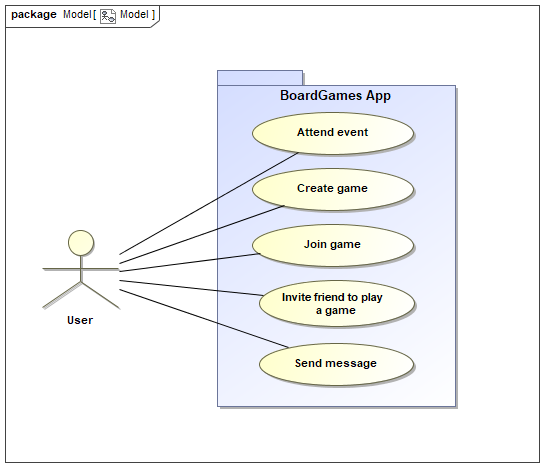
\includegraphics[scale=0.5]{img/UserUseCase}
				\caption{Vartotojo sistemos naudojimo scenarijus}
				\label{img:UserUseCase}
			\end{figure}
			
			\begin{enumerate}
			\item Prisijungti prie žaidimo - vartotojas gali prisijungti prie 
				jau egzistuojančio žaidimo, kuriam įvykti trūksta kelių žaidėjų. (žr. \ref{img:JoinGameSequence} pav.)
				\begin{figure}[H]
					\centering
					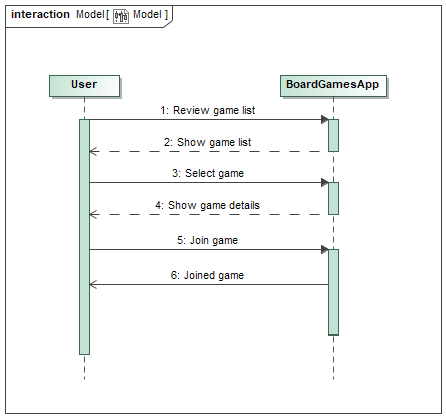
\includegraphics[scale=0.5]{img/JoinGameSequence}
					\caption{Vartotojo prisijungimo prie žaidimo sekų diagrama}
					\label{img:JoinGameSequence}
				\end{figure}
				\textbf{Aprašas:}\\
					Prisijungęs vartotojas gali peržiūrėti jam siūlomus žaidimus, 
					kuriuos yra sukūrę kiti vartotojai. Išsirinkęs žaidimą pagal 
					informaciją, pateiktą su kiekvienu pasiūlymu (žaidimo pavadinimas, 
					vartotojo, sukūrusio žaidimą, vardas ir t.t.), vartotojas jį 
					paspaudžia ir jam parodoma išsamesnė informacija apie žaidimą 
					(jo laikas, vieta, žaidėjų kiekis, aprašymas). Jei visa informacija 
					vartotoją tenkina, jis gali spausti prisijungimo mygtuką. Sistema 
					praneša, apie sėkmingą prisijungimą.
				
			\item Sukurti žaidimą - vartotojas gali inicijuoti privatų arba viešą 
			žaidimą, pasirinkti žaidėjų skaičių, žaidimo vietą, laiką (žr. \ref{img:CreateGameSequence} pav.).
				\begin{figure}[H]
					\centering
					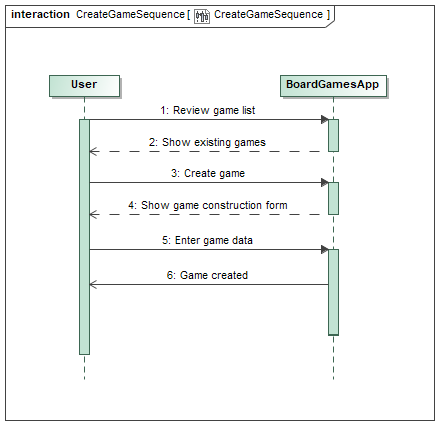
\includegraphics[scale=0.5]{img/CreateGameSequence}
					\caption{Žaidimo kūrimo sekų diagrama}
					\label{img:CreateGameSequence}
				\end{figure}
				\textbf{Aprašas:}\\
					Norėdamas sukurti žaidimą, prisijungęs vartotojas žaidimų sąrašo 
					lange gali pasirinkti kurti žaidimą. Tokiu atveju, jam parodoma 
					žaidimo kūrimo forma, kurioje įrašęs pageidaujamus duomenis 
					(žaidimas, vieta, laikas, žaidėjų skaičius ir t.t), vartotojas ją 
					pateikia. Vartotojas yra informuojamas apie sėkmingą žaidimo sukūrimą.	
					
			\item Pakviesti draugą žaisti - vartotojas gali pakviesti draugą žaisti 
			pasirinktą žaidimą, jei yra pakankamai laisvų vietų (žr. \ref{img:InviteFriendSequence} pav.).
				\begin{figure}[H]
					\centering
					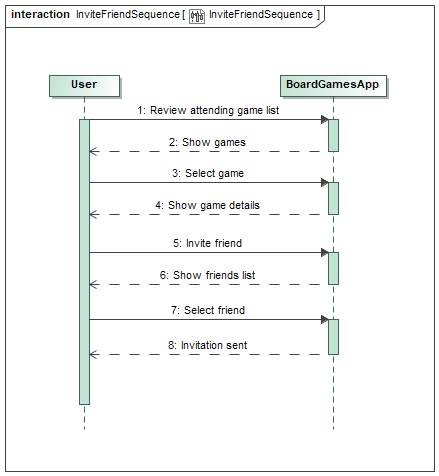
\includegraphics[scale=0.5]{img/InviteFriendSequence}
					\caption{Draugo pakvietimo žaisti sekų diagrama}
					\label{img:InviteFriendSequence}
				\end{figure}
				\textbf{Aprašas:}\\
					Vartotojas, prieš pasirinkdamas prisijungti prie žaidimo, gali 
					pakviesti prie jo prisijungti savo draugą. Vartotojui, 
					pasirinkusiam tam tikrą žaidimą, parodoma platesnė informacija 
					apie jį. Čia vartotojas gali pasirinkti pakviesti draugą - 
					jam parodomas jo draugų sąrašas ir, paspaudus vieną iš draugų, 
					vartotojui pranešama, apie sėkmingą kvietimo išsiuntimą.
				
			\item Parašyti žinutę draugui - vartotojas aplikacijoje gali bendrauti 
			su draugais žinutėmis. (žr. \ref{img:SendMessageSequence} pav.).
				\begin{figure}[H]
					\centering
					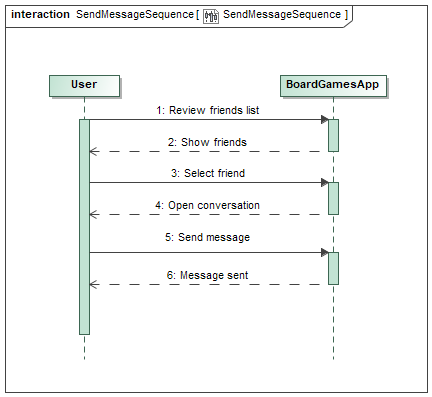
\includegraphics[scale=0.5]{img/SendMessageSequence}
					\caption{Žinutės siuntimo sekų diagrama}
					\label{img:SendMessageSequence}
				\end{figure}
				\textbf{Aprašas:}\\
					Vartotojui suteikiama galimybė peržiūrėti savo draugų sąrašą, 
					pasirinkus vieną ar daugiau draugų, atsidariusiame 
					susirašinėjimų lange, vartotojas gali išsiųsti žinutę.
					
			\item Dalyvauti renginyje - vartotojas gali dalyvauti žaidimų kūrėjų 
			inicijuotame renginyje ar varžybose. (žr. \ref{img:ParticipateEventSequence} pav.).
				\begin{figure}[H]
					\centering
					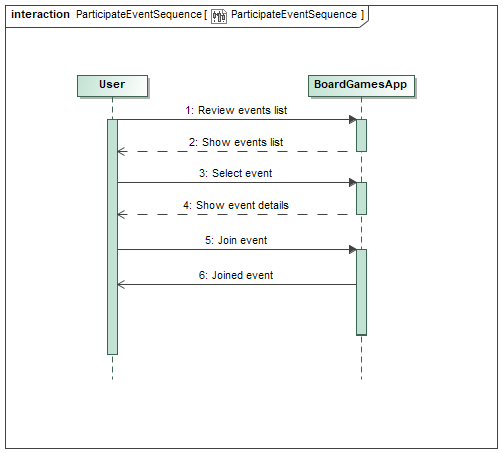
\includegraphics[scale=0.5]{img/ParticipateEventSequence}
					\caption{Vartotojo prisijungimo prie renginio sekų diagrama}
					\label{img:ParticipateEventSequence}
				\end{figure}
				\textbf{Aprašas:}\\
					Vartotojui suteikiama galimybė peržiūrėti savo draugų sąrašą, 
					pasirinkus vieną ar daugiau draugų, atsidariusiame 
					susirašinėjimų lange, vartotojas gali išsiųsti žinutę					
		\end{enumerate}	
		
			
		\subsubsection {Žaidimų kūrėjo}
		\subsubsection {Administratoriaus}
		
	\subsection {Esama būklė}
	Šiuo metu BoardGames komanda turi:
	\renewcommand{\labelitemi}{$\bullet$}
		\begin{itemize}
			\item 5 kompiuterius.
			\item 5 Visual Studio Community programavimo aplinkas.
			\item Telefoną su Android operacine sistema.
			\item Telefoną su IOS.
			\item 3G/4G ryšį mobiliuose įrenginiuose.
			\item Windows forms aplikaciją kūrimo stadijoje.
			\item GitHub repozitoriją.
		\end{itemize}	

	\subsection {Priemonės scenarijui įgyvendinti}
	Priemonės, kurių BoardGames komandai trūksta tikslingam programos įgyvendinimui:
	\renewcommand{\labelitemi}{$\bullet$}
		\begin{itemize}
			\item Privati Git repozitorija.
			\item Duomenų bazė.
			\item Serveris aplikacijos api talpinti.
			\item Patyrę programuotojai aplikacijai sukurti.
			\item Rinkodaros strategija.
			\item Numatytos lėšos aplikacijos talpinimui skirtingų platformų aplikacijų parduotuvėse.
		\end{itemize}		
\end{document}
